\chapter{Context}\label{chap::1}

\vfill

\minitoc

\newpage

\glsresetall

The application of physics concepts and techniques to the field of health-care is nowadays well-established in the clinical routine. Even if physical techniques have been used in medicine from the earliest time\parencite{Duck2014}, the discipline today known as \enquote{medical physics} emerged and grown in the past century thanks to the increasing knowledge and use of ionizing radiations both for diagnosis and disease treatment. In the late \nth{19} century, the x-ray discovery by R\"{o}ntgen, the radioactivity discovery by Henri Becquerel, and the radium and radioactive isotopes studies by Pierre and Marie Curie paved the way to the whole medical physics practice of the next century, where x-ray imaging and radiotherapy were soon established. Following the first successes, more attention were given to radio-protection and dosimetry studies, and the investigations focused on new ways to use radioactive tracers for imaging purpose; this finally led to the birth of nuclear medicine, with the clinical use of the radioisotope \gls{ind131} in 1939~\parencite{Kereiakes1987}. Nuclear medicine rapidly gained importance in the diagnosis clinical panorama, also thanks to the introduction of new detectors, such as the Anger camera introduced in the '60s, and new imaging techniques, such as the detection of photons from positron annihilation (\gls{pet}). Moreover, several alternative methods were proposed or implemented for diagnosis (\gls{mri}, ultrasounds, etc.) and more refined treatment techniques were introduced with the development of particle accelerators after World War 2~\parencite{Keevil2012}.  

At present days, the medical physics progress strongly relies on technological development and computer science, which already revolutionized several fields of science. In particular, cancer research is now a key area for technical and technological development, concerning both diagnosis and treatment\parencite{Webb2009}. Cancer continues to be one of the major issues in the medical scenario: it is at present the second cause of death worldwide, but it is expected to surpass heart diseases and become the main killer in the next tens of years~\parencite{Jemal2010, Thun2010}. The last two decades saw important improvements in radiotherapy techniques and machines, with more precise dose planning and delivery, which enhanced the patient survival and strongly reduced the impact of radiations on healthy tissues. This was possible also thanks to refined imaging technologies, allowing for an accurate tumor volume definition, as well as for image-guided treatments. In this scenario, ion beam therapy, already proposed in the middle of the past century, is rapidly spreading thanks to novel beam delivery technologies, able to relatively reduce the treatment costs and allowing for a commercial diffusion of this treatment method (which is still very limited with respect to standard radiotherapy). Notwithstanding the remarkable steps forward disclosed in the last years, there is still wide room for improvements in this fields, which mainly requires strong imaging basis in order to fully profit of the treatment technique potential.

The work presented in this document have been carried out in this context and deals with the development of gamma imaging detectors to be applied in the field of quality assurance for ion beam treatment. Furthermore, the same detectors have been applied to the nuclear medicine field in simulation, with the aim of assessing its possible clinical implementation for a future development of the nuclear medicine clinical routine. 

In the following sections, a general overview of the two main domains concerned in this thesis work is given, with particular focus on the present status of the involved instrumentation.       
  

\section{Ion beam therapy}\label{chap1::sec::ionBeamTher}

Radiation treatment is an essential component of the tumor therapy, being the second most applied and successful kind of therapy after surgery~\parencite{Schardt2010}. The majority of patiens with localized malignant tumors are treated with radiations~\parencite{Durante2009, Baskar2012, Moding2013}, applied in several fractions in different days in order to reduce the damages to normal tissues~\parencite{Bentzen2006}. The most of the patients treated with radio-therapy techniques receives standard photon treatments, with x-rays coming from linear electron accelerators, while a small percentage undergoes specialized gamma treatments like brachytherapy or gamma knife irradiations. About 1~\% of the radiotherpay patients are irradiated with charged particle beams, with the so-called ion beam therapy~\parencite{Durante2016}.\\
Ion beam therapy, or \enquote{hadrontherapy}, is a cancer radiation treatment method based on light ion beams instead of photons. It was first proposed by Wilson in 1946~\parencite{Wilson1946}; the author highlighted the physical principles and the possible benefits driven by the implementation of such a kind of radiation in clinical treatments, with particular focus on the simple case of protons and some considerations about heavier ions, like alpha particles. At that time, the accelerator technologies were still under development and the treatment required beam energy were about to be reached; the first patients have been treated almost ten years later in the USA by Lawrence and Larson~\parencite{Tobias1955, Tobias1958} with protons and, later on, with He ions~\parencite{Halperin2006}. Nowadays clinical adapted machines are well-established on the market, making ion beam therapy emerging as a wide-spread technique in the every-day cancer treatment routine all over the world. An intense research effort has been dedicated to this field in the last decades; in addition to considerable improvements achieved in the accelerator technologies, new and refined imaging techniques allowed for important enhancement in the treatment planning, also supported by the continuous development of computer science and the growth of calculation power. In parallel, the biological implications of ion irradiation has been deeply investigated~\parencite{Tobias1982, Brahme2004, Friedrich2012, }. Moreover, since more and more patient are treated every year with this technique, more clinical data are at present available for further study and the connection between physicists and physicians is strongly progressing both in the research field and in treatment practice. Several advancements are expected in the next years, following the extensive research work carried out by several groups in the world. In the following paragraph, the basic physical principles and features of this treatment method are explained, and advantages and drawbacks with respect to standard radiotherapy techniques are analyzed. After that, the need of ion range verification is discussed and detailed in order to reach the main topic for this thesis: the prompt-gamma detection.   

\subsection{Physics of ion beam therapy}\label{chap1::subsec::Physics}
High-energy beams of charged nuclear particles show a characteristic depth-dose distribution in matter which makes them suitable for the application in cancer treatment as a valid alternative to standard photon therapy (x-ray or megavolt beams), bringing several advantages to the patient side. The peculiar energy deposition profile (\enquote{Bragg curve}) is named for Sir William Henri Bragg, who investigated the slowing-down process of $\mathrm{\alpha}$ particles in air~\parencite{Bragg1904, Bragg1905}. Low-energy (x-rays) and high-energy photons interacting with the patient body lose their energy according to an exponential attenuation law, with the deposited dose decreasing at increasing depth. Even if high-energy photons can spare the entrance surface thanks to a dose peak shift of a few centimeters (mainly due to forward scattered Compton electrons), a high relative dose is delivered to the tissues along the whole beam path. In order to maximize the tumor volume-to-healthy tissue dose ratio, a standard photon treatment always foresees several irradiation fields from different entrance points and angles (see \figurename~\ref{chap1::fig::XraysCionsFields}). In contrast to photons, the energy deposited per unit track increases for increasing depth for protons and heavier ions; the depth-dose profile is characterized by an entrance low relative dose \textit{plateau} and by a narrow high deposited dose peak at the end of the ion range (in the last few millimeters), called \enquote{Bragg peak}. A visual comparison of low- and high-energy photon, proton and carbon ion relative dose profile in water is given in figure~\ref{chap1::fig::Depth-doseProf}. 

\begin{figure}[!htbp]
\centering
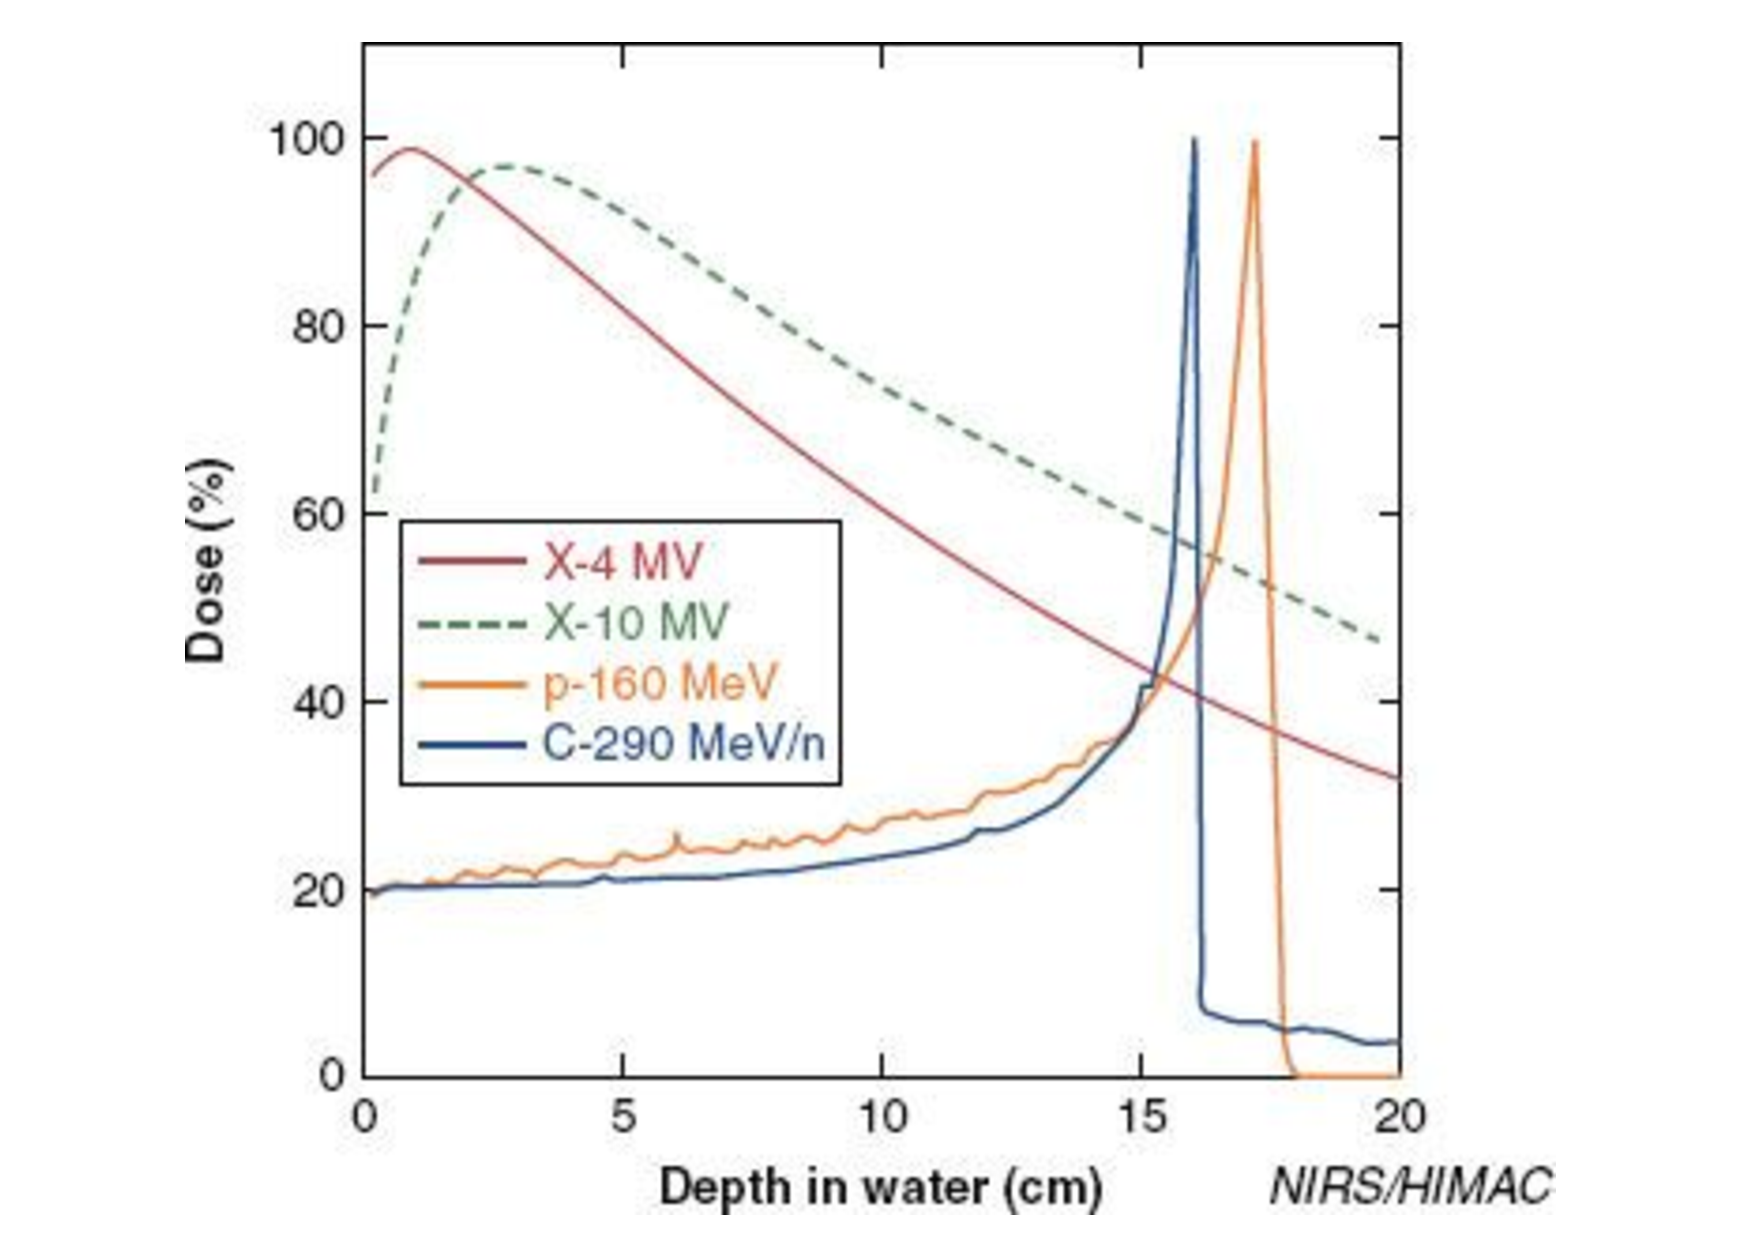
\includegraphics[width=0.6\textwidth]{03_GraphicFiles/chapter1_Introduction/depthDoseProf.pdf}
\caption{Relative dose as a function of the particle depth in water for photons at different energies, protons, and carbon ions.}
\label{chap1::fig::Depth-doseProf}
\end{figure} 

\begin{figure}[!htbp]
\centering
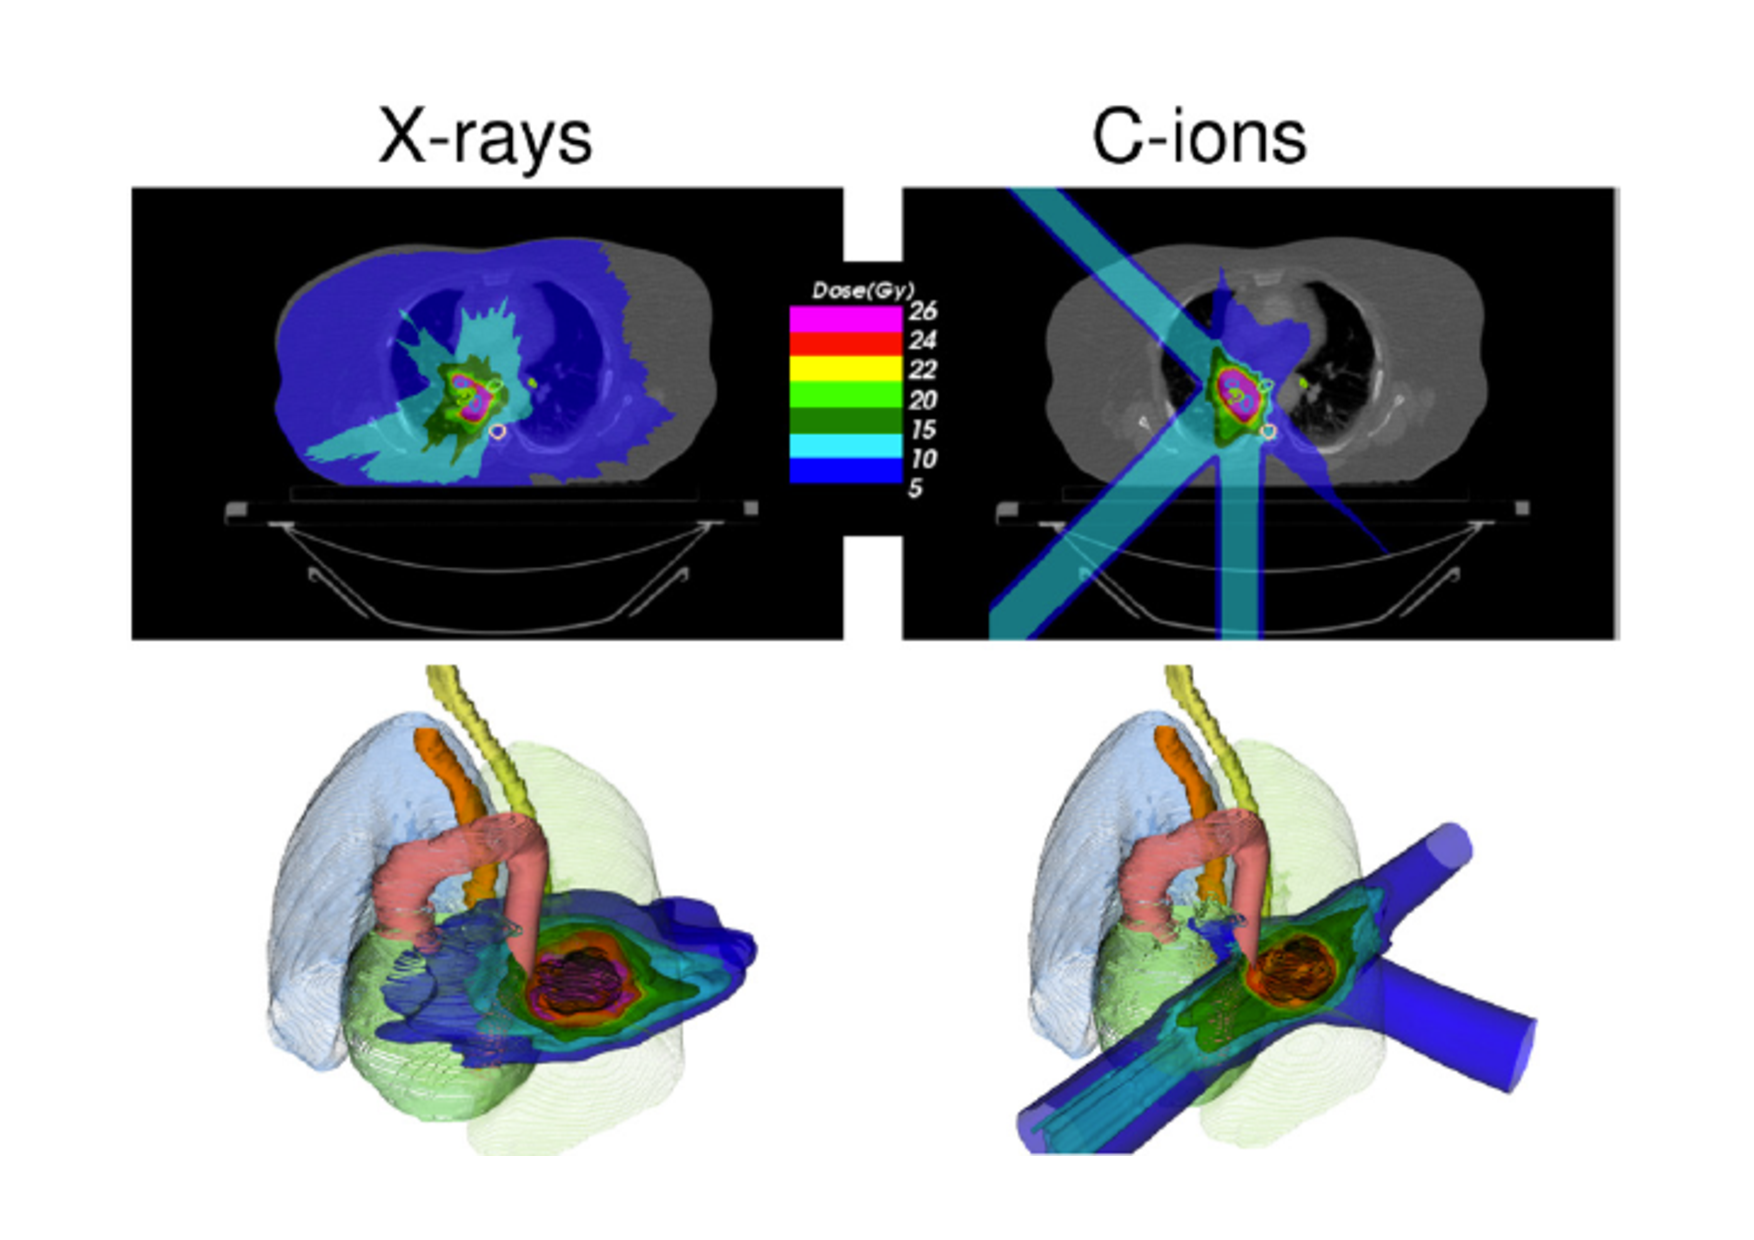
\includegraphics[width=0.6\textwidth]{03_GraphicFiles/chapter1_Introduction/xRayCions_fields.pdf}
\caption{Treatment planning of lung cancer for the irradiation with x-rays (left) or carbon ions (right) (in~\cite{Durante2016}).}
\label{chap1::fig::XraysCionsFields}
\end{figure} 

In order to reach the target volume and deliver the prescribed dose to a tumor inside the patient body, the ions employed in treatment must be accelerated to about 60-70\% of the speed of light ($\beta$ = 0.6-0.7, see~\cite{Durante2016}) via different acceleration techniques and machines, described in section~\ref{chap1::subsec::beamDelivery}. At that energy, the peculiar configuration of the charged particle energy deposition in matter is mainly governed by the energy loss in ionization of the atomic shell electrons, described by the formula attributed to Bethe~\parencite{Bethe1930} and Bloch~\parencite{Bloch1933}, often referred as Bethe-Bloch formula, reported in equation~\ref{chap1::eq::bethe-bloch} in its form independent of the mass density. This expression is also known as mass stopping power.\\
  
\begin{equation}
\frac{S}{\rho} = -\frac{dE}{\rho dx} = 4\piN_{A}r^{2}_{e}m_{e}c^{2}\frac{z^{2}}{\beta^{2}}\frac{Z}{A}\bigg[\ln{\frac{2m_{e}c^{2}\beta^{2}\gamma^{2}}{I}}-\beta^{2}-\frac{\delta}{2}-\frac{C}{Z}\bigg]
\label{chap1::eq::bethe-bloch}
\end{equation}

where $N_{A}$ is the Avogadro's number (6.022 $\times$10$^{23}$mol$^{-1}$), $r_{e}$ is the classical electron radius, $m_{e}$ is the electron mass, $z$ is the charge of the projectile, $Z$ and $A$ are the atomic number and weight of the target material, respectively, $c$ is the speed of light, $\beta = v/c$ is the projectile velocity, $\gamma = (1-\beta^{2})^{-1/2}$, $I$ is the mean excitation potential of the target material. The last two terms represent corrections for high energies ($\delta$ term) and low energies ($C$ term) incident ions. As highlighted in~\cite{Newhauser2015}, the two main parameters governing the projectile energy loss rate in the human body are its velocity (energy) and the the material composition; the density in a patient can vary by almost three orders of magnitude, ranging from the air cavity in the lungs to the most dense bones. 

The energy loss equation directly leads to the definition of the ion beam range in matter, which is the integral over the incident energy of the energy loss per track unit. In general, a \gls{csda} is used for simplicity, assuming a mono-dimensional ion path and an average, continuos energy loss rate. To be noticed that the range is not a deterministic value, but it is intended as an average value and defined for the whole beam, not for single incident particles, which are affected by statistical fluctuations in the energy loss, leading to the so-called range straggling (described by different theoretical models, such as the ones in~\cite{Bohr1915, Landau1944, Vavilov1957}). As realized by Bragg and Kleeman~\parencite{Bragg1905}, the range dependence on the incident particle energy can be practically expressed with the power law in equation~\ref{chap1::eq::rangePowerLaw}

\begin{equation}
R(E) = \alpha E^{p}
\label{chap1::eq::rangePowerLaw}
\end{equation}

where the constant $\alpha$ depends on the target material and the constant $p$ is related to the projectile energy (or velocity) and ranges between 1 and 1.8 in proton-therapy~\parencite{Durante2016}. An empirical expression has been derived to scale the proton calculated range to heavier ions at the same energy per nucleon in the same material: it is reported in equation~\ref{chap1::eq::ScaleRange}.

\begin{equation}
\frac{R_{2}}{R_{1}} = \frac{M_{2}}{M_{1}}\frac{z_{1}^{2}}{z_{2}^{2}}
\label{chap1::eq::ScaleRange}
\end{equation}

with M and z the ion mass and charge, respectively. Equivalently, for the same particle in different material, the scaling formula is reported in equation~\ref{chap1::eq::ScaleRangeMat}.

\begin{equation}
\frac{R_{2}}{R_{1}} = \frac{\rho_{2}}{\rho_{1}}\frac{\sqrt{A_{1}}}{\sqrt{A_{2}}}
\label{chap1::eq::ScaleRangeMat}
\end{equation}
 
 with $\rho$ and $A$ density and atomic mass of the target material, respectively.\\
 It is clear from this considerations that the ion range prediction is affected by uncertainties due to both the target and the projectile feature knowledge: in particular, target composition, mass density and linear stopping power, as well as the beam energy distribution, result in a considerable spread in the beam effective range with respect to the predicted one. In general, the longitudinal beam straggling can be described by a Gaussian function~\parencite{Vavilov1957}, leading to the expression of the relative straggling in equation~\ref{chap1::eq::relStragg}:\\
 
 \begin{equation}
\frac{\sigma_{R}}{R} = (M^{-\frac{1}{2}})\phi\frac{E}{Mc^{2}}
\label{chap1::eq::relStragg}
\end{equation}

The straggling is then all the more reduced as the ion mass increases.

In addition to the overall energy loss considered till here which shapes the beam in the longitudinal direction (range variations),  \gls{mcs} and nuclear interactions play an important role in the resulting beam and dose distribution structure. The \gls{mcs} is determined by elastic electromagnetic interactions of the beam ions with the target nuclei, causing considerable deflections in the single ion trajectory which mainly affect the lateral beam profile causing a spread. Starting from the single scattering model by Rutherford~\parencite{Rutherford1911}, and moving to the calculation of the statistical distribution fucntion for the scattering angle at a certain penetration depth given by~\cite{Bothe1921}, a complete theory allowing for the calculation of the scattering angle probability has been proposed by Moli\`{e}re~\parencite{Moliere1948} (confirmed to provide good predictions thanks to a large set of proton beam spread data - see~\cite{Gottschalk1993}) and then simplified for analytic calculations towards a Gaussian approximation. The Gaussian standard deviation expression in equation~\ref{chap1::eq::latSpread} is given by the characteristics \gls{mcs} angle~\parencite{Highland1975}

 \begin{equation}
\sigma_{\theta} = \frac{14.1 \mathrm{MeV}}{\beta p c}Z_{p}\sqrt{\frac{L}{L_\mathrm{rad}}}\big[1+0.038 \ln\big(\frac{L}{L_{\mathrm{rad}}}\big) \big]
\label{chap1::eq::latSpread}
\end{equation}

where $L$ is the material thickness and $L_{\mathrm{rad}}$ is the radiation length (reported for common materials in~\cite{Tsai1974}). Even if the Gaussian approach is not always accurate to describe the lateral beam spread,  it allows to retrieve the main parameters contributing to this effect: in particular, heavier particles have more narrow lateral beam shape, and the scattering effect increases at increasing ion range (but is inversely proportional to the beam energy) and for high-Z materials. A measurement of the lateral beam spread in a water column for different beam energies (ranges) is reported in~\cite{Pedroni2005}.

In addition to the elastic electromagnetic interactions, primary ions impinging on a target also undergo non-elastic reactions with the target nuclei which may cause the disintegration of the projectile and the target nucleus or a partial frangementation. In general, nuclear reactions induce modifications in the beam composition which must be taken into account for the delivered dose estimate, causing both modification in the longitudinal and lateral beam structure. Moreover, this kind of reactions leads to the production of secondary particles, such as secondary protons, neutrons, hydrogen and helium isotopes and other ions (mainly with heavy ion irradiation), gammas.\\ 
The nuclear interactions occurring between projectile ions and target nuclei are described by a two-step process generally known as abrasion-ablation model~\parencite{Serber1947, Hufner1975}, depicted in \figurename~\ref{chap1::fig::abrAbl}.


\begin{figure}[!htbp]
\centering
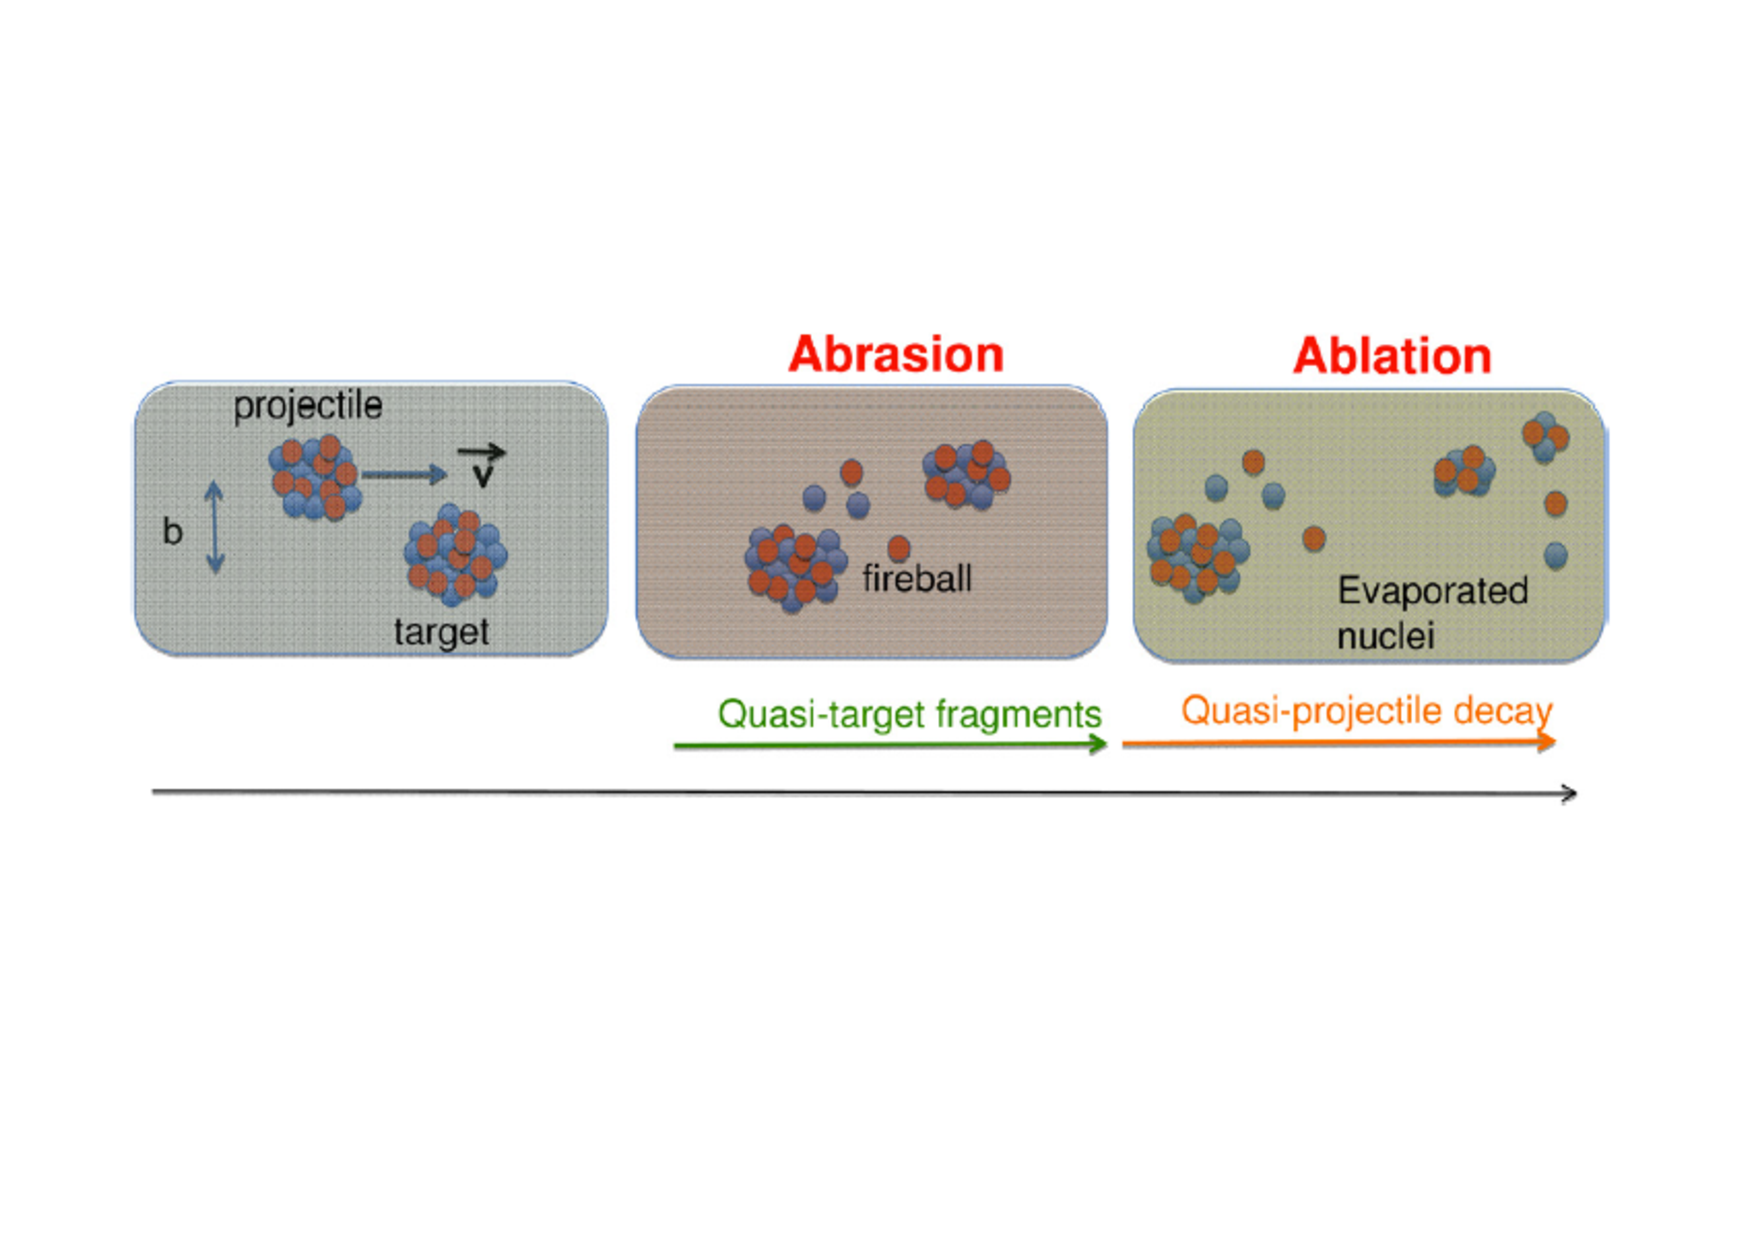
\includegraphics[trim={0 5cm 0 3cm} , clip , width=0.95\textwidth]{03_GraphicFiles/chapter1_Introduction/AbrasionAblation.pdf}
\caption{Schematic view of the abrasion-ablation model for the description of ion-nucleus interactions (in~\cite{Durante2016}): b is the distance between projectile center and target nucleus center, v is the projectile velocity.}
\label{chap1::fig::abrAbl}
\end{figure} 

Depending on the distance between projectile and target centers, named $b$, a variable number of nucleons is involved in the interaction and composes the reaction zone generally defined \enquote{fireball}. This nucleons are abraded in the first interaction step, while the \enquote{spectator} nucleons are almost not affected. During the second step, the fireball de-excites in an evaporation process. With increasing penetration depth, the increased number of nuclear reactions causes a growing loss of primary particles with the consequent production of lower-Z fragments. It is clear that peripheral collisions (high $b$) lead to smaller loss of primaries with respect to central collision (small $b$), where projectile and target are most likely completely destroyed. \figurename~\ref{chap1::fig::nuclearReacLoss} shows the primary particle fluence loss in a proton beam as a function of the depth in water~\parencite{Newhauser2015}. In the entrance region before the falloff the fluence loss is caused by nuclear reaction, while close to the Bragg peak the fluence falloff is mainly due to absorption of primary particles which limited residual energy. In addition, the range straggling effect is visible. Concerning carbon ion beams, as reported in~\cite{Durante2016}, during a standard treatment only 50\% of the primary ions reaches the Bragg peak region, while the others are undergo fragmentation processes.\\ 
The projectile velocity determines the velocity of the secondary fragments, which can travel with longer ranges with respect to the primaries due to their reduced mass: this produces a tail in the dose distribution (for ions heavier than protons). The features of this tail have been deeply studied for different primary ions species ($^{10}$B, $^{12}$C, $^{14}$N, $^{16}$O, $^{20}$Ne), and shell-structure effects have been verified with a non-direct relationship between proton number Z and tails extension~\parencite{Schall1996}.  \figurename~\ref{chap1::fig::TailBragg} show the effects of nuclear reactions on the Bragg curves related to carbon ion beams at different energies stopping in water, measured in a water column~\parencite{Schardt2008}.  With increasing primary energy and, consequently, beam penetration depth, the ratio between Bragg peak and entrance plateau dose is reduced by the decreased number of primary ions, while the tail after the Bragg peak is wider due to the increased number of lower-Z fragments traveling with longer range. In addition to this, the energy loss stochastic fluctuations is clearly visible in the broadening of the Bragg peak.  

\begin{figure}
\begin{subfigure}[t]{.5\textwidth}
\centering
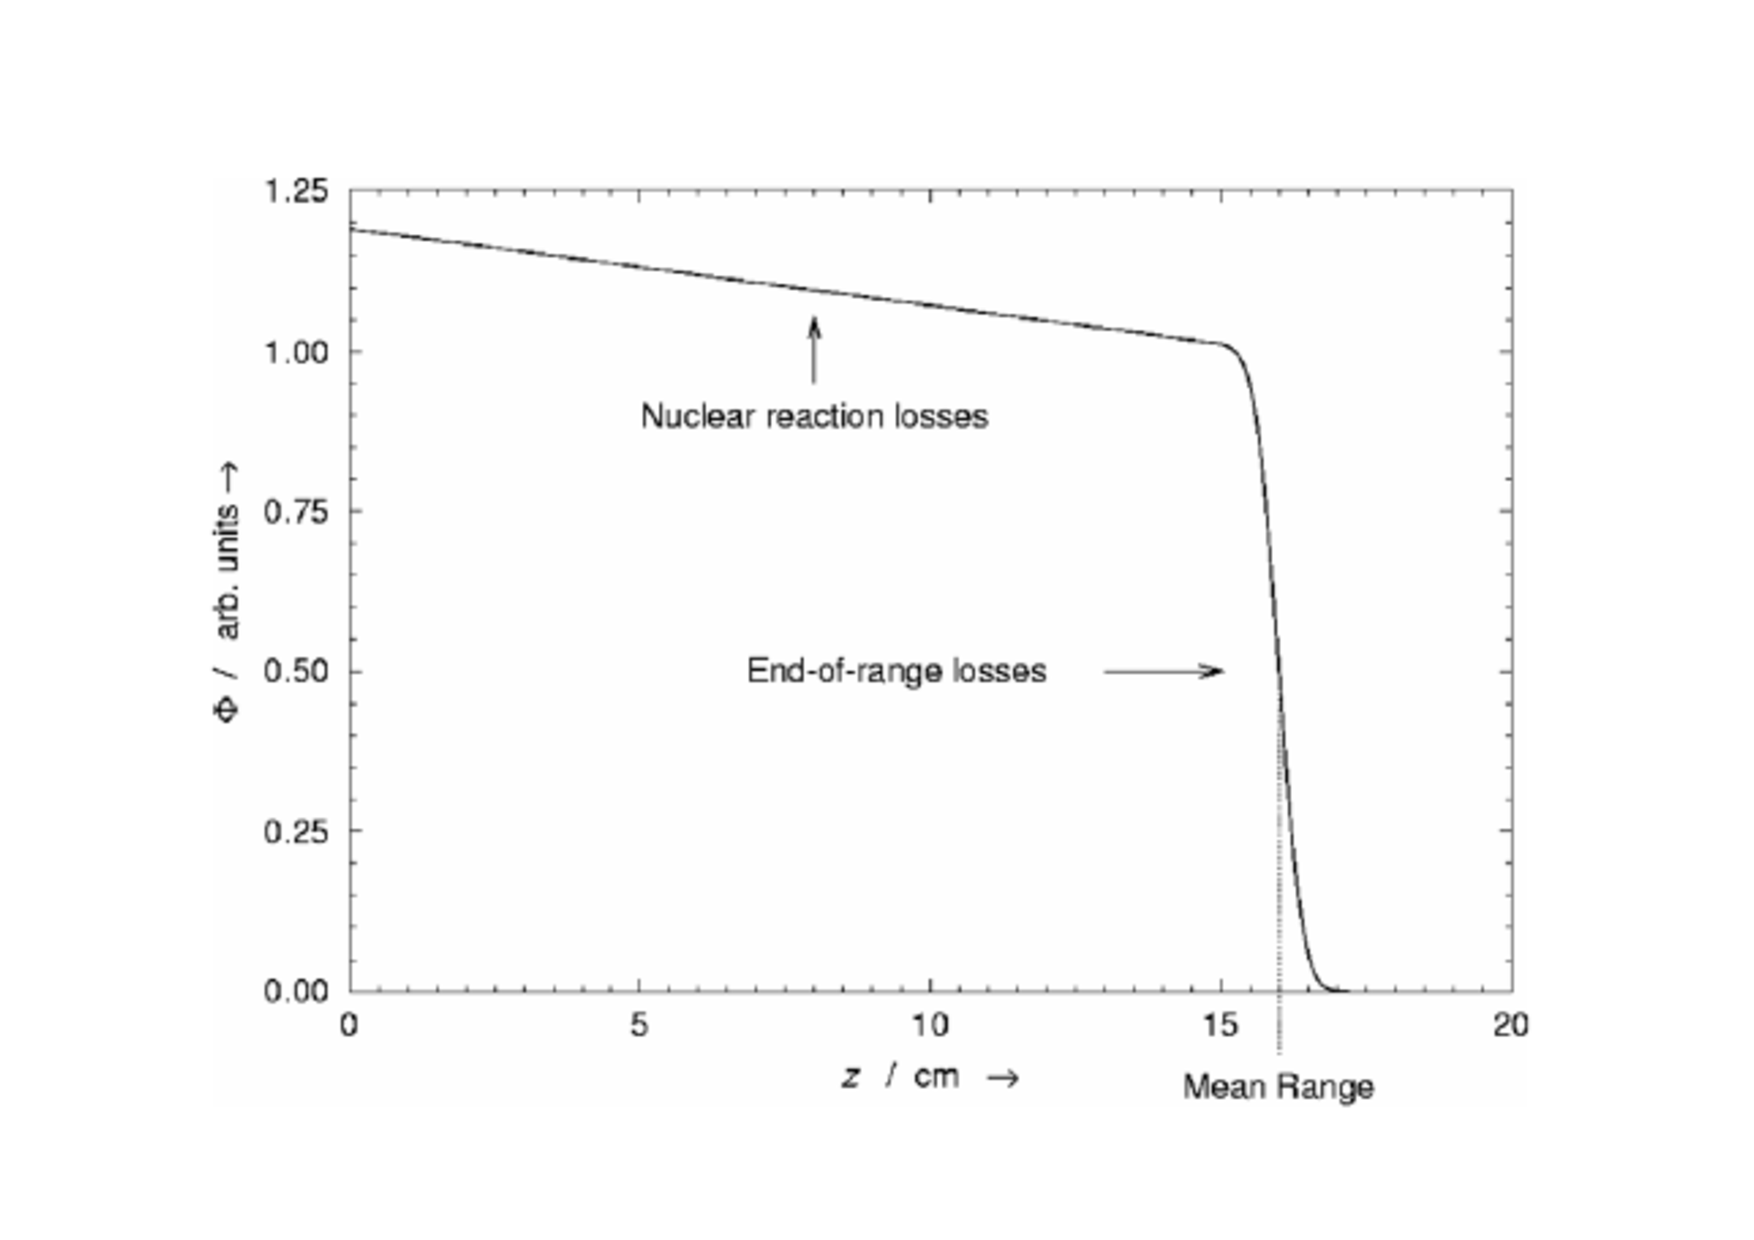
\includegraphics[width=1.\textwidth]{03_GraphicFiles/chapter1_Introduction/primaryLoss.pdf}
\caption{Primary particle fluence loss in a proton beam as a function of the depth in water (in~\cite{Newhauser2015}).}
\label{chap1::fig::nuclearReacLoss}
\end{subfigure}
\begin{subfigure}[t]{.5\textwidth}
\centering
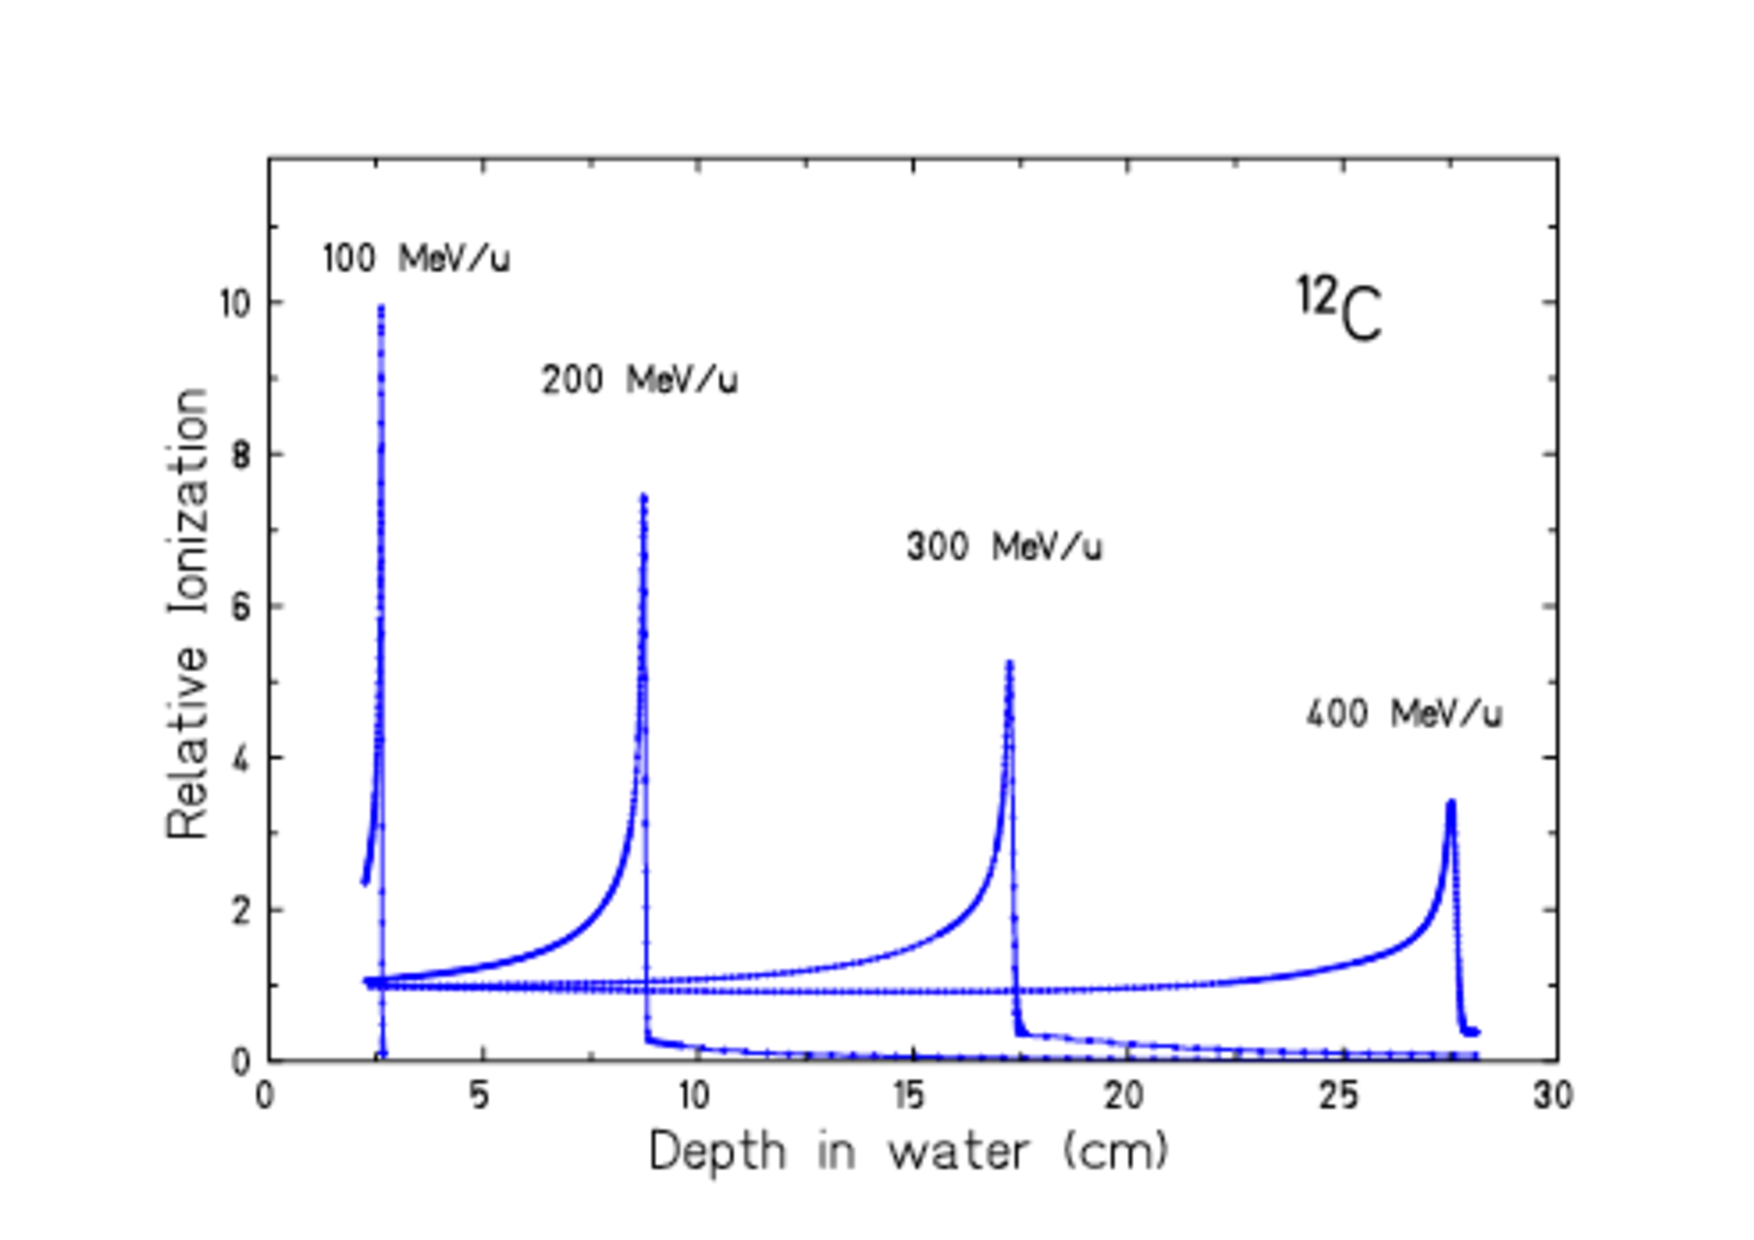
\includegraphics[width=0.92\textwidth]{03_GraphicFiles/chapter1_Introduction/tailBragg.pdf}	
\caption{Measured relative ionizations for carbon ion beams stopping in water (in~\cite{Schardt2008}).}
\label{chap1::fig::TailBragg}
\end{subfigure}
\caption{Effects of nuclear interactions on the primary beam and resulting dose distribution.}
\label{chap1::fig::}
\end{figure}

Further, interesting results about ion fragmentation in nuclear interactions can be found in~\cite{Matsufuji2003, Wroe2005, Haettner2006, Gunzert-Marx2008, Haettner2013}.\\

Detailed information about fragmentation can be retrieved via Monte Carlo simulations and used to evaluate the impact on the delivered dose. As an example, simulations published in~\parencite{Grassberger2011} of 160~MeV protons in water allowed to estimate the dose contributions given by primary particles (between 90\% and more than 99\% of the total depending on the range), with the remaining fraction of dose mainly connected to secondary protons and $\alpha$ particle: negligible dose is given by heavier fragments. A more intense dose contribution from heavier fragments is expected for carbon ion irradiation, but an accurate Monte Carlo simulation of these processes is still a challenge. \\
As mentioned, in addition to charged fragments, nuclear interactions also produce gammas, mainly originating from atomic de-excitation processes (prompt-gammas) or from the annihilation of positron emitted by beta-emitter fragments ($^{10}$C, $^{11}$C, $^{13}$N, $^{14}$O, $^{15}$O), and neutrons. All the secondary particles which can be absorbed by the target contribute to the total dispensed dose to the target, while the others (except neutrons), escaping the target volume, can be exploited for non-invasive measurements of beam and target features. In particular, different techniques have been proposed and tested to measure secondary protons and gamma rays (both prompt-gammas and positron-annihilation gammas) with the aim of retrieving information about the ion range and obtain an online treatment verification. A detailed  discussion about this topic will be given in section~\ref{chap1::subsec::secondaryRad}.\\
Focusing on neutrons, which are produced in large quantities and over a wide energy range, they must be modeled with care in order to evaluate the safety measures to be implemented in treatment centers~\parencite{Newhauser2002}, as well as the implications in the delivered dose and secondary cancer probability~\parencite{Newhauser2011}. The dose contribution caused by secondary neutrons strongly depends on the beam delivery system (see section~\ref{chap1::subsec::beamDelivery} for the description of the beam delivery systems), as demonstrated in~\cite{Gottschalk2006}. In particular, passive elements used for beam shaping have been identified as one of the main source of secondary neutrons contributing to the total delivered dose to the patient~\parencite{Yan2002}, so that in modern facilities deflecting elements are set after the passive modules in order to limit the neutron flux towards the target. It is interesting to notice that the amount of produced neutrons and resulting dose is compatible for protons and carbon ion irradiation, even if the neutron yield is higher for carbon ions: this is due to the different beam intensities used in clinics for the two species, with more than a factor 20 in favour of protons. Finally, if compared to photon standard radiotherapy, the neutron dose associated to ion beam therapy treatments results to be smaller, as demonstrated in recent studies~\parencite{Schneider2015}.\\

\subsection{Biological effects of ion beam therapy}\label{chap1::subsec::bioEffects} 

In addition to the already presented physical differences between photon radiation therapy and ion beam therapy treatments, a fundamental aspect of the game lies in the biological effect of such radiations. In the following, the main biological implications of radiation therapy are summarized with the aim of highlighting the favorable contribution given by charged particles with respect to photons and, at the same time, discuss some controversial points~\parencite{Paganetti2013}.\\
  

Absorbed dose, defined in ~\cite{ICRU1980, ICRU1998} as 

\begin{equation}
\mathrm{D} = \frac{d\overline{\epsilon}}{dm}
\label{chap1::eq::AbsDoseDef}
\end{equation}

where $d\overline{\epsilon}$ is the mean energy imparted by ionizing radiation to matter of mass $dm$. To be precise, the imparted energy must also be defined: in the same ICRU reports we find that 


\begin{equation}
\epsilon = R_{\mathrm{in}} - R_{\mathrm{out}} + \sum{Q}
\label{chap1::eq::impEnergyDef}
\end{equation}

with $R_{\mathrm{in}}$ and $R_{\mathrm{out}}$ the sum of the energies of all ionizing particles entering or leaving the volume, respectively, $ \sum{Q}$ the sum of all changes of the rest mass energy of nuclei and elementary particles in any nuclear transformations occurred in the volume due to the ionizing radiation.

LET TO BE DEFINED: number of ionizations which radiation causes per unit distance as it traverses the target.

In order to transfer the experience from photon data to ion irradiation and to create a common evaluation parameter, the \gls{rbe} has been introduced and defined as the ratio between the photon and ion equivalent dose:\\

\begin{equation}
\mathrm{RBE} = \frac{D_{\mathrm{photon}}}{D_{\mathrm{ion}}}
\label{chap1::eq::rbeDef}
\end{equation}

where $D_{\mathrm{photon}}$ and $D_{\mathrm{ion}}$ are the absorbed dose for photon and ion irradiation causing the same biological effect. Notwithstanding the apparently simple definition, \gls{rbe} results to be a very complex quantity, but for the moment the only one really used in clinics: it depends on the particle type, energy, on the biological target, as well as on dose and \gls{let}.

\subsection{Advantages and drawbacks with respect to standard radiotherapy}\label{chap1::subsec::ProContro}

%In order to accurately predict the ion range and dose distribution delivered during a clinical treatment, all the possible ion interactions in matter must be considered. 
%From the clinical point of view, all the physical effects described in the previous paragraphs affect the delivered dose distribution and may cause deviations from the planned treatment. Ideally speaking, a perfect knowledge of the beam and target structure and perfect evaluation of all the parameters involved in the dose determination would result in the optimal way to treat a deep-seated tumor, with a reduced dose delivered to the surrounding healthy tissue (even close to \gls{oar}) with limited fields of irradiation, and a dose accurately concentrated to the tumor volume. The actual clinical routine must face limitations in beam production and control as well as in patient composition evaluation, which causes the need for approximated treatment planning and the setup of treatment safety margin. limiting the full exploitation of this treatment technique potential. Starting from the physical principles discussed in this section, in the following paragraph a summary of the main advantages and drawbacks of ion beam therapy with respect to standard photon radiotherapy is provided. More details about the physics of proton and, more generally, ion beam therapy, can be found in~\parencite{Lomax2009, Belkic2010, Schardt2010, Bichsel2013, Nupecc2014,  Newhauser2015, Durante2016}.        


\subsection{Beam delivery}\label{chap1::subsec::beamDelivery}

\subsection{Treatment planning}\label{chap1::subsec::treatmentPlan}

\subsection{Quality assurance in ion beam therapy}\label{chap1::subsec::IonQA}

\subsection{Ion range verification}\label{chap1::subsec::rangeVer}

\subsection{Secondary radiation techniques}\label{chap1::subsec::secondaryRad}

\subsubsection{Positron Emission Tomography}\label{chap1::subsec::RangePET}
\gls{pet} is at present the only method clinically implemented for ion range verification~\parencite{Hishikawa2002, Enghardt2004, Parodi2007, Bauer2013}. \gls{pet} techniques are based on the detection of the two back-to-back 511~keV photons produced by the annihilation of positrons (created by the emitter fragments of nuclear reactions) with patient electrons, resulting in a delayed radiation which should be detected with time coincidences, allowing for an intrinsic background reduction. Nevertheless, the monitoring with positron emitters secondary signal must deal with a limited count rate compared to medical imaging PET, with the lifetime of emitters providing a delayed information that implies the signal integration over a whole treatment fraction (not a single spot or group of spots), with physiological washout effects depending on the emitters lifetime.

Even if the only available and functional range monitoring system in a clinical center is based on this technique~\parencite{Enghardt2004}, several clinical experience with commercial or adapted PET system already shown intrinsic limitations mainly connected to the ring geometry (not directly applicable to the treatment monitoring due to the presence of the beam) or in general to geometrical constraints limiting the field of view and the resulting system global efficiency and spatial accuracy (the limited detection angle generates artifacts in the final image)~\parencite{Parodi2016}. The research is ongoing and new results are expected for the next years thanks to the introductions of new systems with adapted geometries, to the improvements in acquisition and reconstruction techniques and to the clinical introduction of time-of-flight systems, intrinsically able to improve the detector spatial resolution via interaction time information, and depth-of-interaction reconstruction, which will allow for a more precise spatial reconstruction for reduced angular artifacts effects.

%\subsection{Prompt-gammas: physics and features}



%\subsection{State of the art of range verification and prompt-gamma techniques}


\section{Nuclear medicine}\label{chap1::sec::NuclearMed}


\subsection{PET and SPECT}\label{chap1::subsec::PET-SPECT}


\subsection{State of the art of PET and SPECT}


\clearpage
%\printbibliography[heading=subbibintoc]
